\section{Results and discussion}

\subsection{Benchmarks and verification} \label{sec:res_benchmarks}

\subsubsection{Benchmarks for the brute force approach, no repulsion or jastrow factor}
Table \ref{tab:N2_norep} shows the results from the brute force simulation of the two electron - no repulsion case. 
A plot of the results is shown in figure \ref{fig:N2_norep}. 

\begin{table}[h!]
	\centering 
	\begin{tabular}{l @{ } l @{ } l @{ } l @{ } l @{ } l @{ } l @{ } l @{ } l @{ } l @{ } l @{ } l @{ } l @{ } l @{ } l @{ } l @{ } l @{ } l}
		\toprule
		$\alpha~~~~$ & $0.0~~~~$ & $0.05~~~~$ & $0.1~~~~$ & $0.15~~~~$  & $0.2~~~~$ & $0.25~~~~$ & $0.3~~~~$ & $0.35~~~~$ & $0.40~~~~$ & $0.45~~~~$  \\
		\shaderow $E$(a.u) & 1.1e5 & 19.96 & 10.03 & 6.77 & 5.17 & 4.23 & 3.61 & 3.19 & 2.89 & 2.66  \\ 
		$\textrm{Variance} ~~$ & 7.4e9 & 2.0e2 & 4.8e1 & 2.0e1 & 1.1e1 & 7.0e0 & 4.5e0 & 3.1e0 & 2.2e0 & 1.5e0  \\ 
		\midrule
		$\alpha~~$ & $0.5~~$ & $0.55~~$ & $0.6 ~~$  & $0.65 ~~$ & $0.7~~$ &  $0.75~~$ & $0.8~~$ & $0.85~~$  & $0.9~~$ & $0.95~~$ \\
		\shaderow $E$(a.u.) & 2.49 & 2.36 & 2.26 & 2.18 & 2.12 & 2.08 & 2.047 & 2.024 & 2.0096 & 2.002 \\ 
		$\textrm{Variance}$  
		& 1.1e0 & 7.9e-1 & 5.6e-1 & 3.9e-1 & 2.6e-1 & 1.7e-1 & 1.0e-1 & 5.3e-2 & 2.6e-2 & 5.2e-3 \\
		\midrule
		$\alpha~~$ & $1.0~~$ & $1.05~~$ & $1.1~~$ & $1.15~~$  & $1.2~~$ & $1.25~~$ & $1.3 ~~$  & $1.35 ~~$ & $1.4 ~~$ & $1.45~~$ \\ 
		\shaderow $E$(a.u) & 2 & 2.0029 & 2.010 & 2.021 & 2.035 & 2.05 & 2.07 & 2.09 & 2.12 & 2.14 \\ 
		$\textrm{Variance}$ & 3.3e-13 & 4.7e-3 & 1.8e-2 & 3.9e-2 & 6.7e-2 & 1.0e-1 & 1.4e-1 & 1.8e-1 & 2.3e-1 & 2.9e-1 \\ 
	\bottomrule
	\end{tabular}
	\caption{Table showing the results from the brute force VMC simulation of the expectation value of the local energy $\langle E_L \rangle$ for $\alpha$ between $0$ and $1.45$ in the 2-electron case with no repulsion or Jastrow factor. 
	The results show a minimum for the energy at $\alpha = 1$, as expected, and the variance at this point is so small that we expect it to be an eigenstate of the system.}
	\label{tab:N2_norep}
\end{table}


\begin{figure}[h!]
	\centering 	
	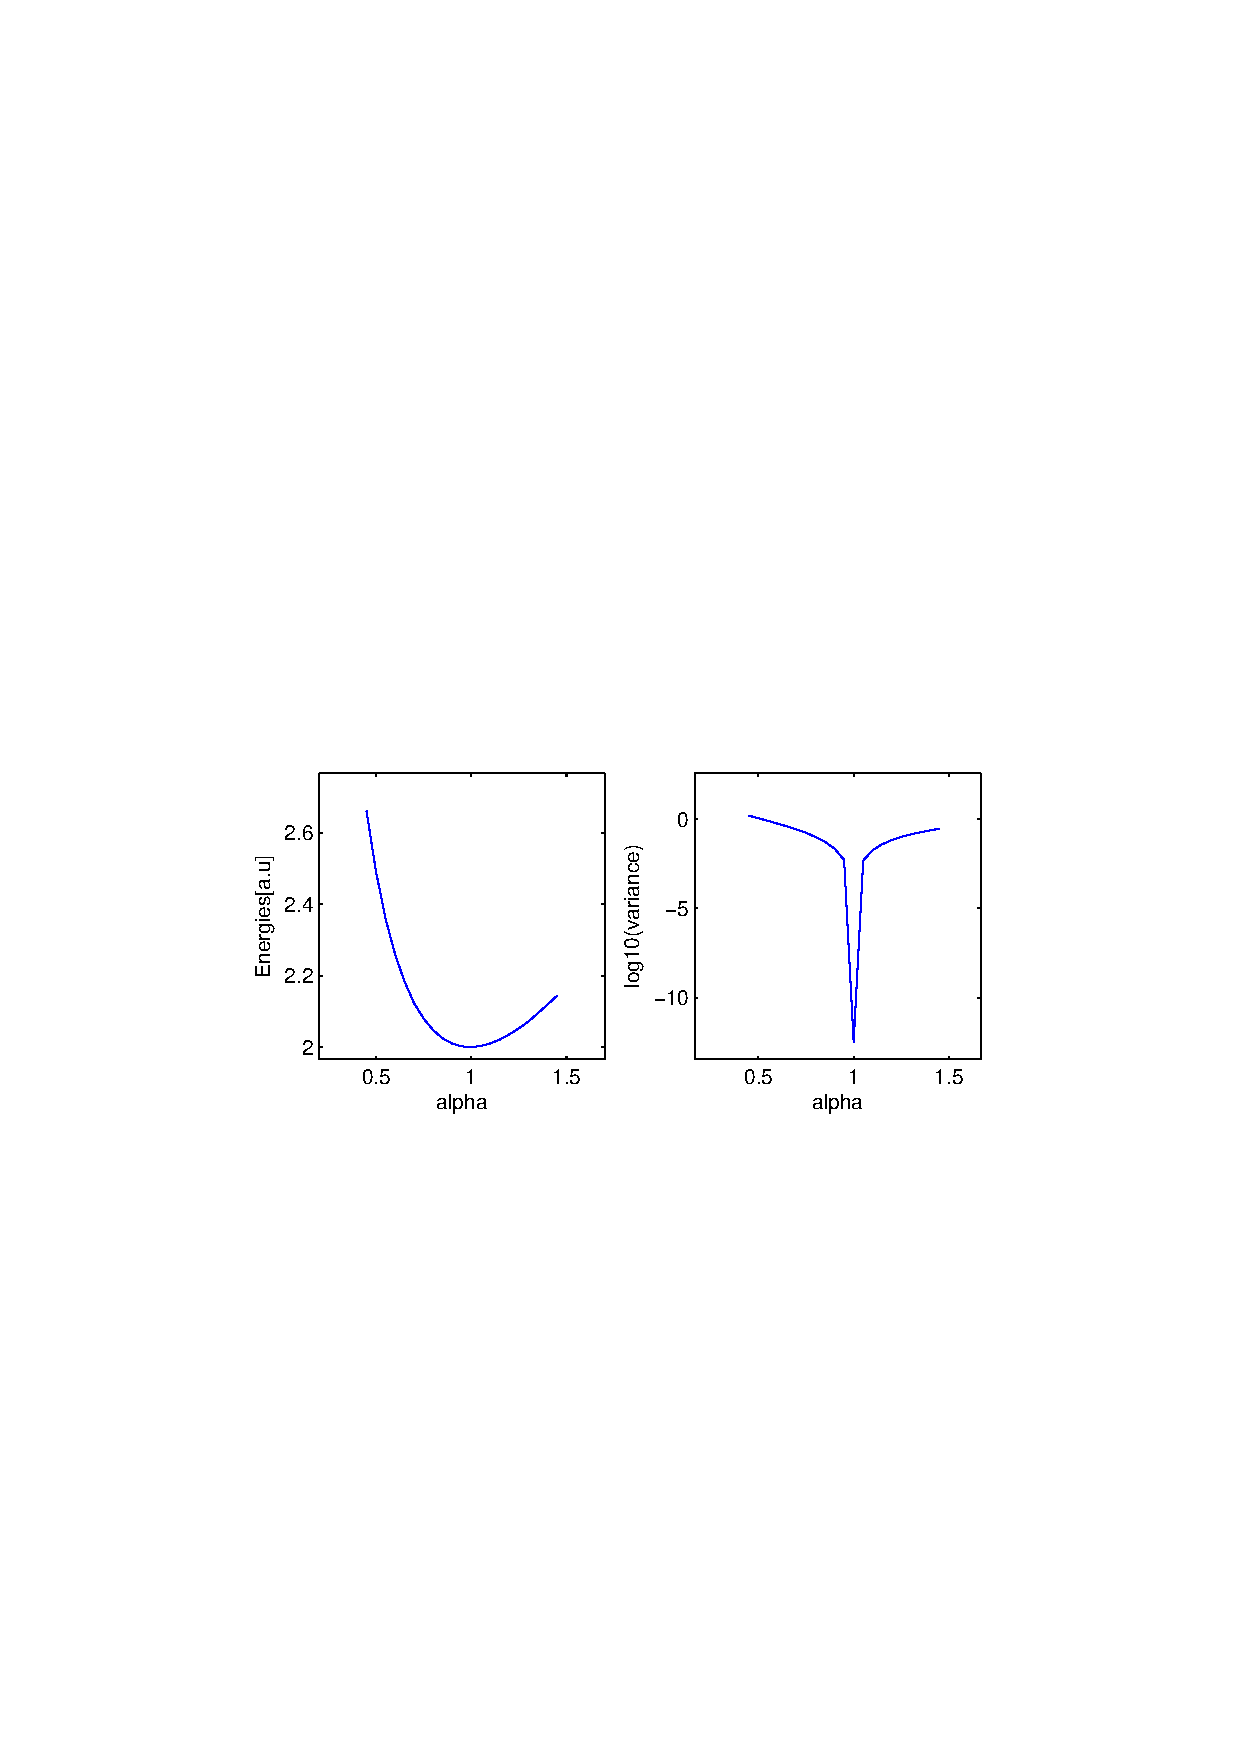
\includegraphics[width=\textwidth]{results/N2_norep.jpg}
	\caption{Plot of the values given in table \ref{tab:N2_norep}, the brute force VMC simulation of the two-electron no repulsion or Jastrow factor case. 
	Some of the first values of $\alpha$ has been omitted to make the graph more informative.}
	\label{fig:N2_norep}
\end{figure}

The figure shows exactly what we would expect from the discussion of section \ref{sec:motivation}. 
The energy is always larger than $2$ a.u. and takes this value only when $\alpha = 1$. 
We also see a huge drop in the variance just as we reach $\alpha = 1$ which indicates that this is indeed an eigenstate of the system.
What little is rest of the variance at $\alpha=1$ can be due to numerical errors in the calculation of the laplacians. 
This has in retropspect been verified to be true by using the analytical expression for the local energy. 

Table \ref{tab:N6_N12_norep} shows the result from the $N=6$ and $N=12$ electrons case with no repulsion using the brute force approach with numerical evaluation of the local energy.

\begin{table}[h!]
	\centering 
	\begin{tabular}{l @{}l @{ } l @{ } l @{ } l @{ } l @{ } l}
		\toprule
		\multirow{3}{*}{N=6}$~~\quad ~~$ & $\alpha~~~~$ & $0.9~~~~~~~~~~~~~$ & $0.95~~~~~~~~~~~~~$ & $1~~~~~~~~~~~~~$ & $0.105~~~~~~~~~~~~~$  & $0.11$ \\
		 & $E$(a.u) & 15.0803 & 15.0850 & 15 & 15.0184 & 15.0708\\ 
		 & $\textrm{Variance} ~~$ & 2.49e-1 & 5.89e-2 & 2.56e-13 & 2.36e-2 & 2.05e-1\\ 
		\midrule
		\multirow{3}{*}{N=12} & $\alpha~~~~$ & $0.9~~~~$ & $0.95~~~~$ & $1~~~~$ & $0.105~~~~$  & $0.11$ \\
		& $E$(a.u) & 42.2114 & 42.0497 & 42 & 42.0563 & 42.1937 \\ 
		& $\textrm{Variance} ~~$ & 6.92e-1 & 1.66e-1 & 1.72e-10 & 1.48e-1 & 5.69e-1\\ 
		\bottomrule
	\end{tabular}
	\caption{The results from calculating the expectation value of the local energy and its variance.
			We see that the code works for the $N=6$ and $N=12$ case because we are producing the expected results, $E_6 = 15$ and $E_{12} = 42$ ($\omega = 1.5$). 
			The variance at $\alpha=1$ is so small that we have probably the exact wavefunction.}
	\label{tab:N6_N12_norep}
\end{table}

The table shows that we are able to produce the results we anticipated.
What little there is of variance at $\alpha=1$ is probably due the numerical evaluation of the local energy, which has been confirmed in retrospect by using the analytical expression for the local energy. 
It also shows that the code has implemented the oscillator frequency $\omega$ correctly. 

\subsubsection{Benchmark for the brute force approach, with repulsion and jastrow factor}

A plot of the energies and $log_{10}$ of the variances after the investigation is shown in figure \ref{fig:N2_rep}.

\begin{figure}[h!]
	\centering
	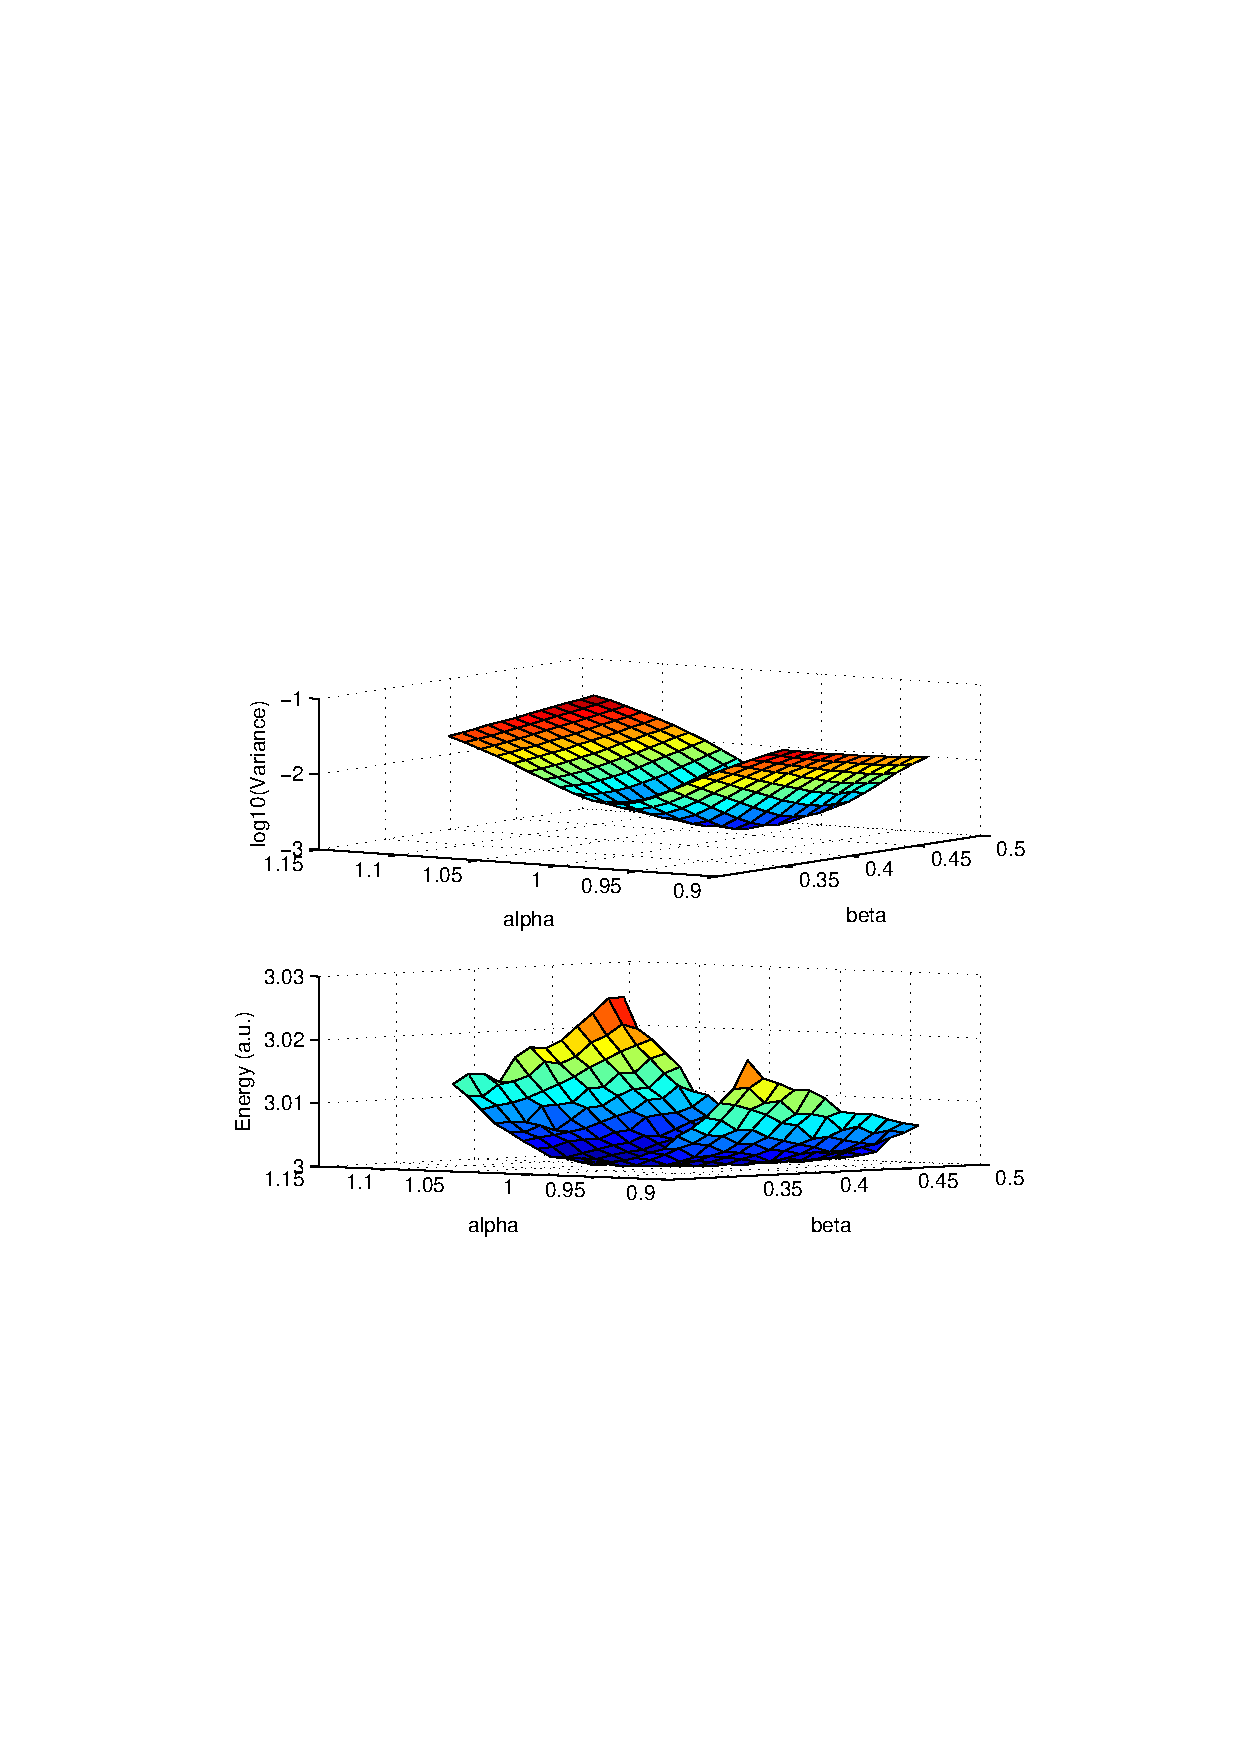
\includegraphics[width=\textwidth]{results/N2_rep.jpg}
	\caption{Plot of the expectations of the local energy and $log_{10}$ of variances after the VMC simulations with two electrons, with repulsion and jastrow factor. 
	Each point was based on $10^6$ simulations. 
	The figure gives an overview of how the energies vary as function of $\alpha$ and $\beta$.
	The lowest energy $E= 3.00022$ where $\alpha = 0.98$ and $\beta = 0.42$.}
	\label{fig:N2_rep}
\end{figure}

It is not easy to see from the figure what is the lowest energy, but manipulating the figure in matlab revealed the smallest test state energy, which is given in table \ref{tab:N2_rep}.

\begin{table}[h!]
		\centering 
	\begin{tabular}{l}
		\toprule
		The lowest energy $E=3.00022$ and $\textrm{Variance} = 0.001568$ at $\alpha = 0.98$ and $\beta = 0.42$. \\
		\bottomrule
	\end{tabular}
	\caption{The lowest energy found from the VMC study of the two electron case with repulsion and Jastrow factor.}
	\label{tab:N2_rep}
\end{table}

The lowest energy was also found in the region where the variance was lowest. 
It seems thus that the value obtained in this VMC calculation was very close to the real lowest eigenstate. 
Very close, however, does not mean that we have found \textit{the} eigenstate. 
As we saw in the previous section, when we hit the real eigenstate, the variance dropped rapidly to sizes in order of magnitude $10^{-12}-10^{-13}$ which was not the case here. 



\subsubsection{Comparison of different methods}

The results from calculation $\langle E \rangle$ for the different method combinations and problem/wave function parameters are shown in table \ref{tab:methods_E}.

\begin{table}[h!]
	\centering
	\begin{tabular}{l @{ } l @{ } l @{ } l @{ } l @{ } l @{ } l  @{ } l  @{ } l  @{ } l }
	\toprule
	  & \multicolumn{3}{c}{Problem and Wavefunction parameters} \\
	 Method parameters $~~~~$ & (2, 1, Jf, 0, 1, Ef) $~$ & (12, 0.5, Jf, 0, 1.5, En) $~$ & (6, 0.82, Jo, 0.22, 3, En)  \\
	\midrule
	(BF, NLE) & 				(2.000, 6e-13)		&		(92.10, 67.54)		&		(54.74, 28.11)			\\
	\shaderow (BF, ALE)	 &		(2.000, 0)			&		(92.18, 161.4)		&		(54.72, 28.19)		\\
	(IS, NLE,NQF) & 			(2.000, 6e-14)		&		(92.15, 66.43)		&		(54.72, 27.33)				 \\
	\shaderow(IS, NLE, AQF) &	(2.000, 1e-13) 		&		(92.06, 54.49)		&		(54.72, 27.32)						\\
	(IS, ALE, NQF) &			(2.000, 0)			&		(92.13, 143.2)		&		(54.76, 27.35)					\\
	\shaderow (IS, ALE, AQF) &	(2.000, 0) 			&		(92.12, 76.24)		&		(54.74, 27.44)	 				\\
	\bottomrule
	\end{tabular}
	\caption{A table of the expectation value and variance (Energy, Variance) of the local energy obatined with different Problem/Wavefunction parameters (N,$\alpha$, Jn/Jf, $\beta$, $\omega$, En/Ef). For explanation of abbreviations, see section \ref{sec:exp_methods_E}.
	For all trials, $10^6$ VMC calculations were performed and for the importance sampling methods, a timestep of $\delta t = 0.1$ was used.}
	\label{tab:methods_E}
\end{table}

These are very strong results. 
Firstly, we have verified the nummerical brute force method against known benchmarks and seen that they are correct,
thus, it seems that the other methods are working properly!
Secondly, the different methods used very different ways to obtain the results. 
That the results are almost the same is a strong indication that all the methods are doing the same thing and working correctly. 

\subsection{Optimizations and differences} \label{sec:res_opt_and_diff}

\subsubsection{Test cases}

The results from finding the optimal parameters for $\alpha$ and $\beta$ for the different test cases are given in table \ref{tab:test_cases}.

\begin{table}[h!]
	\centering 
	\begin{tabular}{c  c c  c  c  c  c }
	\toprule
	 Test cases: 			& \multicolumn{2}{c}{$\omega=0.01$} & \multicolumn{2}{c}{$\omega=0.28$} & \multicolumn{2}{c}{$\omega=1$} \\
	 Optimal parameters  	& No Jast. & 	Jast. & No Jast. & 	Jast. & No Jast. & Jast. \\
	 \midrule
	 $\alpha$& 	0.0 & 	0.9 & 	0.6 & 	1.0 	& 0.8	& 1\\
	 $\beta$ & 	- & 	0.07 & 	- & 	0.25 & -  & 0.42\\
	 \midrule
	 Energy (a.u.) & 				0.081 &		0.074 &	 1.14  &	1.00022 & 3.15 & 2.9999 \\
	 Variance & 					1.5e-3 &	1.27e-5	 & 0.42 &	 9.9e-4 & 2.02 & 2.7e-3 \\
	 \bottomrule
	\end{tabular}
	\caption{The optimal parameters with and without Jastrow factor (Jast.).}
	\label{tab:test_cases}
\end{table}

\subsubsection{Jastrow factor}

\subsubsection{Importance sampling}

\subsubsection{Timely differences between methods}













\subsection{Applications}

\subsubsection{Energies and variances}

\subsubsection{The virial theorem }